\documentclass[12pt]{article}
\usepackage{geometry} 
\geometry{margin=1in}
\geometry{a4paper} 


\usepackage{textcomp}
\usepackage{booktabs}
\usepackage{array}
\usepackage{paralist}
\usepackage{verbatim} 
\usepackage{subfigure}
\usepackage{graphicx,caption}
\usepackage{placeins}
\usepackage{lipsum}
\usepackage{xcolor}
\usepackage{dcolumn}
\usepackage{sectsty}
\allsectionsfont{\sffamily\mdseries\upshape}
\usepackage{gensymb,amsmath,mathtools,amssymb}
\usepackage{flafter}
%\usepackage{parskip}
\usepackage[utf8]{inputenc}
\usepackage[english]{babel}
\usepackage{tocbibind}
\usepackage[toc,page]{appendix}
\captionsetup{width=\linewidth}
\usepackage{bm}
\usepackage{hyperref}
\usepackage{siunitx}

\newcommand{\half}{\frac{1}{2}}


\graphicspath{{./figs/}}


\title{Tank Sizing \\ ICE-Cube}
\author{Devansh Agrawal}
%\date{} 


\begin{document}

\maketitle


\section{Introduction}

The design of the tank for the ICE cube thruster system could benefit from optimal sizing of tanks to reduce the system mass. Geometric programming is used to find a optimal solution, implemented using the python package GPkit~\cite{gpkit}. The system is composed of:
\begin{itemize}
\item Main water tank, storing 0.35~L of water at 4~bars. There is a diaphragm holding the pressurant (Helium) away from the water.
\item Pressurant tank, storing the Helium at some arbitrary pressure and temperature, within bounds. 
\end{itemize}

The model here does not include the piping, regulators, temperature regulators. It imposes only rudimentary dimensional constraints to ensure the components can fit in a 1U module. The detailed placement and sizing are to be considered later.

The model does include the mass of the Helium and water and tank masses. It minimises the total mass of the system. 

\section{Tank Stress Model}

A ellipsoid tank is modelled, as this reduces stress concentrations at the seams associated with cylindrical tanks. Fig.~\ref{fig:diagram} shows a representative tank and its dimensions. The spherical cap tank, (where $a = b$) is a degenerate case of the ellipsoid tank. 

%\FloatBarrier
\begin{figure}[htbp]
   \centering
   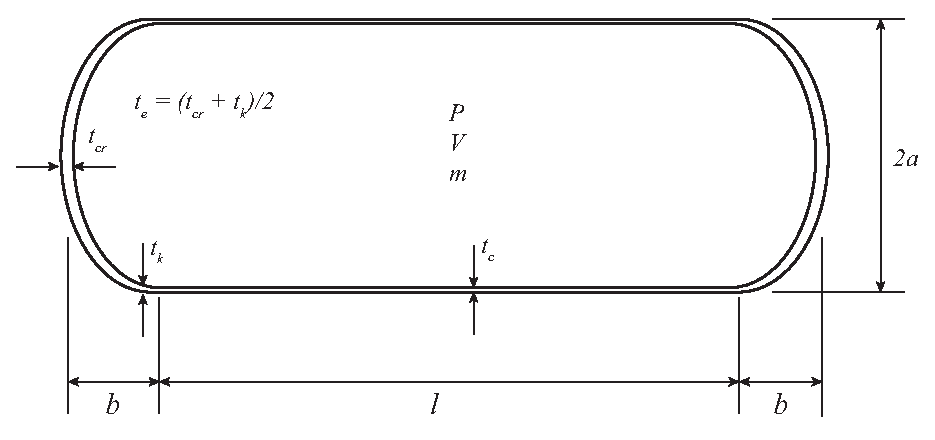
\includegraphics[width=0.7\linewidth]{diagram.eps}
   \caption{Nomenclature of ellipsoid tank. $t_e$ is the effective ellipsoid cap thickness. $P$ is the internal gauge pressure, $V$ is the internal volume.}
   \label{fig:diagram}
\end{figure}
%FloatBarrier

Following Huang~\cite{huang1992}, we can find the tank's internal volume.

\begin{align}
V_\text{tank} &= 2V_\text{ellipsoid} + V_\text{cylinder}\\
&= 2 \frac{2 \pi a^2 b}{3} + \pi a^2 l\\
&= \frac{4 \pi a^3}{3k} + \pi a^2 l
\end{align}

where we use $k= a/b$ as a  the ellipse ratio. 

The wall thickness are sized by the maxim stress in the material. As a safety factor, I assumed the max stress allowed is the lower value of the yield and ultimate strengths of aluminium divided by a safety factor, 
\begin{equation}
\sigma = \min \left(\frac{\sigma_y}{1.1}, \frac{\sigma_u}{1.25}\right)
\end{equation}

The wall thicknesses required are

\begin{align}
t_c &= \frac{Pa}{\sigma e_w}\\
t_k &= \frac{KPa}{\sigma e_w}\\
t_{cr} &= \frac{Pka}{2\sigma e_w}\\
t_e &= \frac{t_{k}+t_{cr}}{2} =  \frac{Pa}{2\sigma e_w} \left(K + \frac{k}{2}\right)
\end{align}

where $t_e$ is the effective wall thickness used for weight estimations and $e_w$ is the weld efficiency, assumed to be 1. The parameter $K$ is the stress factor indicated in Fig.~\ref{fig:stressFactor}, and for compatibility with GPkit, bound by 
\begin{equation}
K \simeq 0.52 k + 0.16
\end{equation}

%\FloatBarrier
\begin{figure}[htbp]
   \centering
   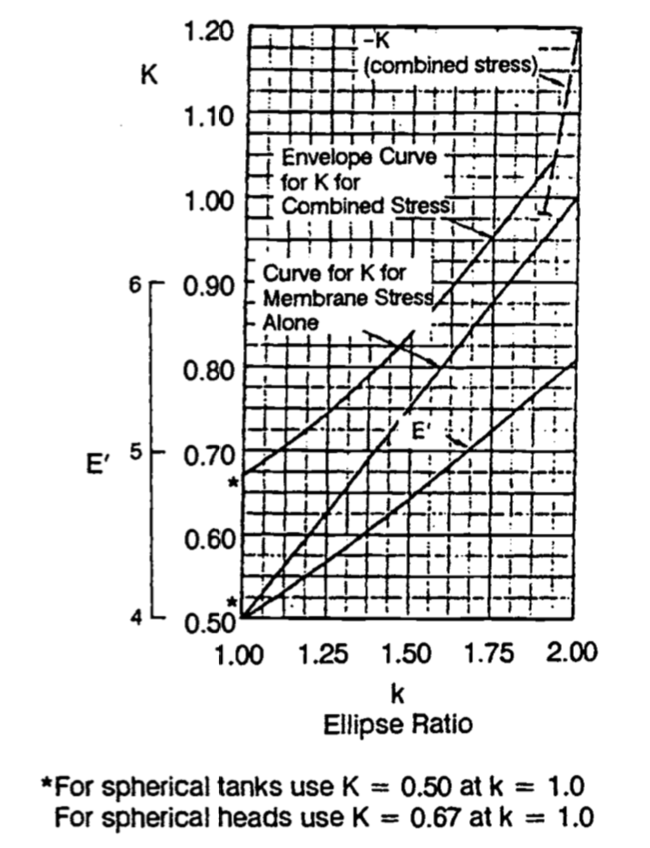
\includegraphics[width=0.5\linewidth]{stressFactor}
   \caption{Stress Factor $K$, and surface area factor $E'$ from \cite{huang1992}.}
   \label{fig:stressFactor}
\end{figure}
%FloatBarrier

The total mass of the tank can be estimated by 
\begin{align}
m_\text{tank} &= 2 m_{ellipsoid} + m_{cylinder}\\
&= 2 \frac{\pi a^2 t_e E' \rho}{2k} + 2\pi a l t_c \rho
\end{align}

where $\rho$ is the tank material density, $E'$ is a surface area factor, as seen in Fig.~\ref{fig:stressFactor}. The explicit expression of $E'$ can be approximated using a series expansion about $k=1.5$ to make it GP compatible,

\begin{align}
E'  &= 2 k+\frac{1}{\sqrt{k^{2}-1}} \ln \frac{k+\sqrt{k^{2}-1}}{k-\sqrt{k^{2}-1}}\\
&= 4.72164+1.53404 (k-1.5)+0.150079 (k-1.5)^2+O\left((k-1.5)^3\right)\\
&= 0.150079 k^2+1.0838 k+2.75826
\end{align}

These relationships were implemented in GPkit, along with the ideal gas law on Helium to size the tanks. 

\section{Optimization Results}

If we allow the helium tank to be at a lower temperature than the main water tank (limited to 100~K), we get the results in Table~\ref{tbl:optimalParams}. However, since the helium pressure is rather high, and the wall thicknesses rather low, we can constrain them and determine a new optimal design. For this example, the $P_{He}< 20$~bar and $t>0.2$~mm for all wall thicknesses. 

It is apparent that the mass of the system is extremely low. The pressures and thicknesses constraints should be refined based on handling requirements. Furthermore, ullage and pipe loses have not been considered at the moment, but can easily be incorporated into the current model. 

Manufacturing constraints have not been considered at the moment, in particular it is not clear how to create these tanks as they are. 



\begin{table}[htbp]
\centering
\caption{Sizing results. The first column applies no additional constraints, while the second requires $P_{He}< 20$~bar and $t>0.2$~mm.}
\begin{tabular}{@{} lrSSl @{}}
\toprule
{Component}  & {Parameter} & {Unconstrained}  & {$P, t$ limited} &{Unit}\\ 
\midrule
Helium Tank & $P$ & 29.28 & 20 & bar\\
	& $T$ & 100 & 100 & K\\
	& $V$ & 15.94 & 23.33 & cm$^3$\\
	&$a$ & 0.8835 & 1.227 &  cm\\
	&$b$& 0.8835 & 0.6134& cm\\
	& $l$ & 2.757 &2.06 &  cm\\
	& $t_c$ & 0.1043  &0.2  & mm\\
	& $t_{cr}$ & 0.05216 & 0.2  & mm\\
	& $t_k$ & 0.07093   & 0.2 & mm\\
	& $t_e$ & 0.06154  & 0.2 &  mm\\
	& $m$ & 0.5938 & 1.563 & g\\
Main Tank & $P$ & 4 & 4 & bar\\
	& $T$& 300 & 300 & K \\
	& $V$ & 350 & 350 & cm$^3$\\
	& $a$ & 3.071 & 3.025 &  cm \\
	& $b$ & 3.071 & 1.513 & cm\\
	& $l$ & 3.857 & 5.08  & cm \\
	& $t_c$ & 0.04954 &0.2  &mm \\
	&$  t_{cr} $ & 0.02477  & 0.2 &mm \\
	&$ t_e $& 0.02923 & 0.2  &mm \\
	&$t_k $& 0.03369 & 0.2  &mm \\
	& $m$ & 1.929 & 9.505& g\\
Helium & $m$ & 0.2247  & 0.2247 & g\\
Water & $m$ & 350 & 350 & g\\
\midrule
Total & $m$ & 352.7 &  361.3 &g\\
	      \bottomrule
\end{tabular}
\label{tbl:optimalParams}
\end{table}

%\FloatBarrier
\begin{figure}[htbp]
   \centering 
   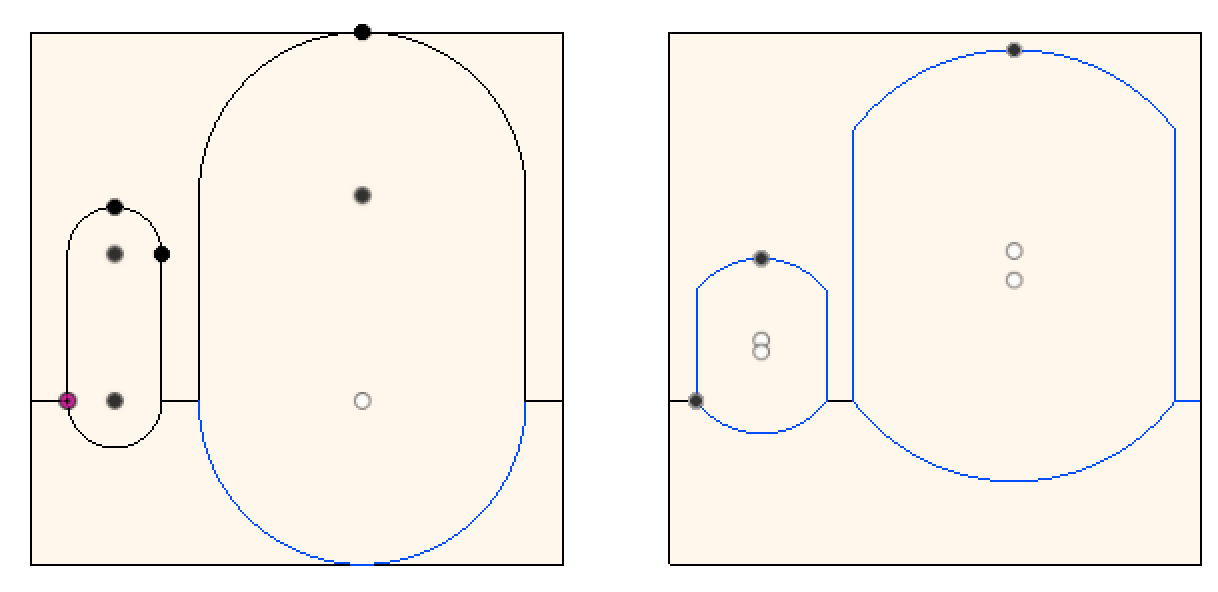
\includegraphics[width=0.8\linewidth]{He_tank_sketch}
   \caption{Sketch of tanks (with Helium pressurant), for the unconstrained case (left) and the constrained case (right). Large squares show 10~x~10~cm square}
   \label{fig:}
\end{figure}

\section{Pressurising using a self-pressurant gas}


In the previous section, we see that the dry mass is on the order of 2-10~grams, the system mass might be dominated by the additional components, for example regulators, valves, temperature control units, piping, etc. This motivates a design that uses a self-pressurising gas, in the appropriate temperature ranges. While I have not yet done an extensive search of such pressurants, one possible choice is a mixture of butane and propane. 

Fig.~\ref{vapour_pressure} shows the vapour pressure from a range of temperatures. Since our target tank pressure is 4~bars, using this combination allows for some flexibility in the vapour pressure between 0 and 20~deg C. A feedback loop with a water pressure sensor can be used in the final implementation to accurately maintain the water pressure. 


%\FloatBarrier
\begin{figure}[htbp]
   \centering
   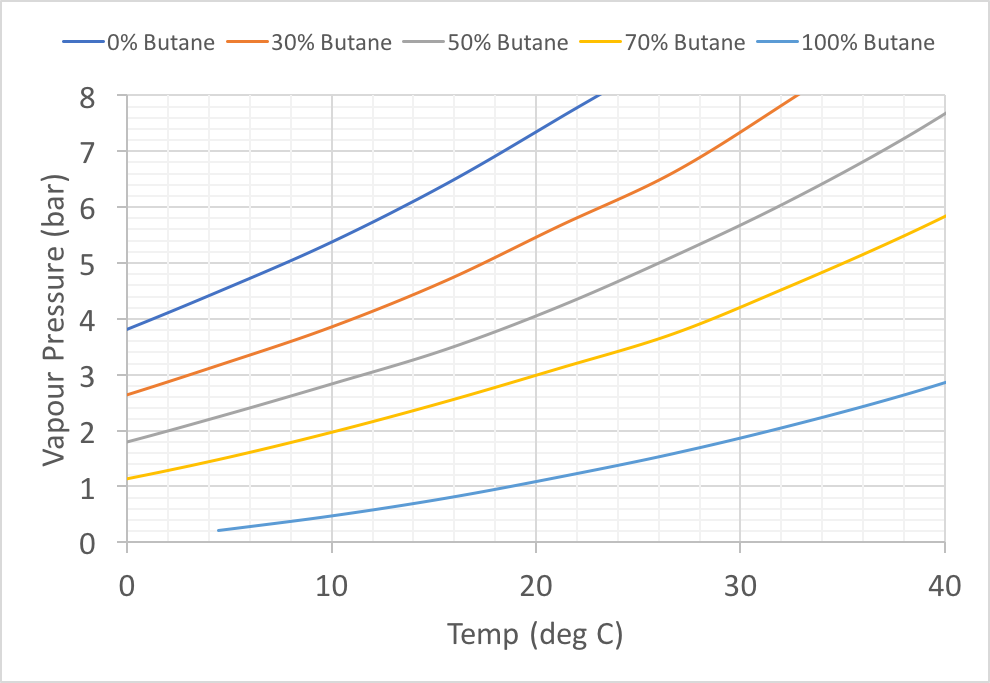
\includegraphics[width=0.7\linewidth]{vapour_pressure}
   \caption{Vapour pressure as a function of temperature and butane-propane molar mix ratio. Recreated from \cite{vapourPressure_engToolbox}, but the more reliable results based on Lange~\cite{lange} were used for sizing.}
   \label{fig:vapour_pressure}
\end{figure}
%FloatBarrier

A low order sizing is needed to estimate the mass of pressurant needed in this situation. From Lange's Handbook of Chemistry~\cite{lange}, we can estimate the partial vapour pressure of butane and propane using the following equation:
\begin{equation}
\log_{10}{P} =   A - \frac{B}{t+C}
\end{equation}
where $P$ is the partial pressure in mmHg, $t$ is the temperature in deg C, and A, B, C are empirical constants:

\begin{table}[htbp]
   \centering
   \caption{Empirical constants of butane and propane}
   \begin{tabular}{@{} lSSSS @{}}
      \toprule
       Species & A & B & C & {Molar mass (g/mol)}\\
      \midrule
Butane & 6.80896 & 935.86 & 238.854 & 58.12\\
Propane & 6.80338 & 804.00 & 247.04 & 44.10\\
      \bottomrule
   \end{tabular}
   \label{tbl:empiricalConstants}
\end{table}

Since the total vapour pressure of a mixture is simply the sum of the partial pressures weighted by the mole fraction, we can find the mole fractions of butane ($x$) and propane $(1-x)$ required,

\begin{align}
P_\text{tank} &= P_\text{butane} + P_\text{propane}\\
& = x P_\text{butane, x=1} + (1-x) P_\text{propane, x=0}\\
&= x \times 10^{\left(A_b - \frac{B_b}{t+C_b}\right)} + (1-x) \times 10^{\left(A_p - \frac{B_p}{t+C_p}\right)}\\
\end{align}

Therefore, $x = (0.195,  0.480, 0.690)$ for temperatures 0, 10, 20 degC. 

Picking 10 degrees C as a reference, we get  partial pressures of $P_\text{butane} = 0.7148$~bar, $P_\text{propane} = 3.28513$~bar. Since we require the vapour to completely displace the water, the volume is 0.35~L, and so we can determine the mass of butane and propane needed in the gaseous phase using the ideal gas law,
\begin{equation}
P_b V = \frac{m_b}{M_b} RT \text{ and } P_p V = \frac{m_p}{M_p} RT
\end{equation}

therefore,
\begin{align}
m_b &= 0.586\text{ g}\\
m_p &= 2.154\text{ g}\\
m_b + m_p = 2.740\text{ g}
\end{align}

which, considering the liquid densities gives a volume of $4.674$~cm$^3$. As the pressurant must have both liquid and gas at all times, some spare quantity of the liquid mixture must be included. 

If we perform an optimal sizing on this system (adding 25\% extra pressurant), we get the results in Table~\ref{tbl:optimalParams_self_pressurisation}.



\begin{table}[htbp]
\centering
\caption{Sizing results if a self-pressurizing tank is used. The first column applies no additional constraints, while the second requires $t>0.2$~mm.}
\begin{tabular}{@{} lrSSl @{}}
\toprule
{Component}  & {Parameter} & {Unconstrained}  & {$t$ limited} &{Unit}\\ 
\midrule
Main Tank & $P$ & 4 & 4 & bar\\
	& $T$& 300 & 300 & K \\
	& $V$ & 355.843 & 355.843 & cm$^3$\\
	& $a$ & 3.111 & 3.042 &  cm \\
	& $b$ & 3.111 & 1.521 & cm\\
	& $l$ & 3.778 & 5.108  & cm \\
	& $t_c$ & 0.05018 &0.2  &mm \\
	&$  t_{cr} $ & 0.02509  & 0.2 &mm \\
	&$ t_e $& 0.02960 & 0.2  &mm \\
	&$t_k $& 0.03412 & 0.2  &mm \\
	& $m$ & 1.971 & 9.611& g\\
Pressurant & $m$ & 3.426  & 3.426 & g\\
Water & $m$ & 350 & 350 & g\\
\midrule
Total & $m$ & 355.4 &  363.0 &g\\
	      \bottomrule
\end{tabular}
\label{tbl:optimalParams_self_pressurisation}
\end{table}

%\FloatBarrier
\begin{figure}[htbp]
   \centering
   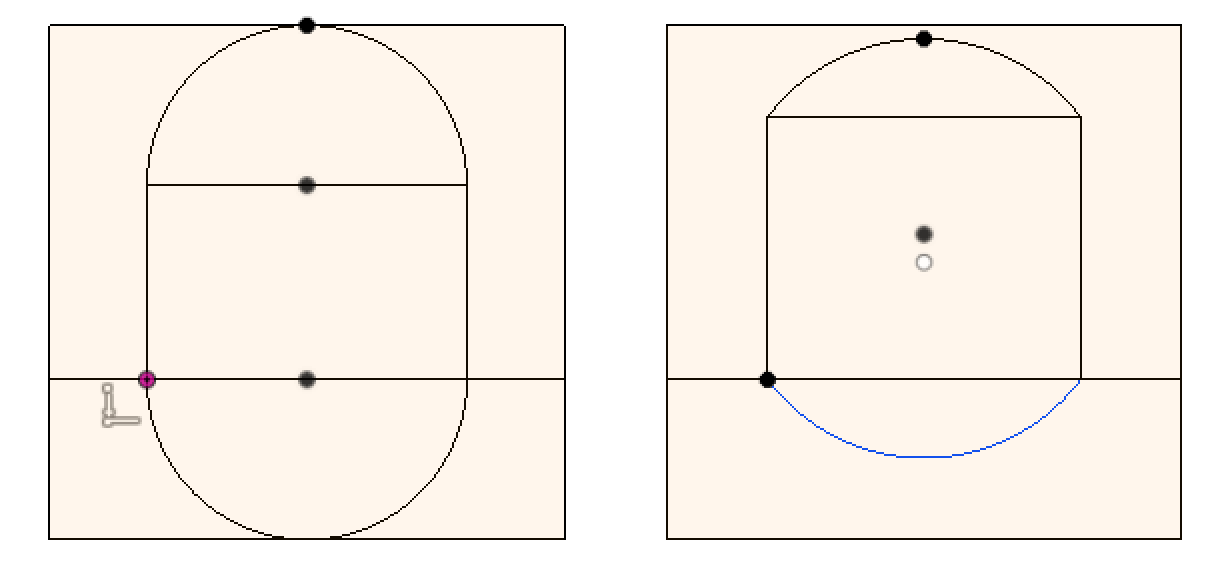
\includegraphics[width=0.8\linewidth]{Butane_tank_sketch.png}
   \caption{Sketch of tank (self pressurising), for the unconstrained case (left) and the constrained case (right). Large squares show 10~x~10~cm square}
   \label{fig:}
\end{figure}
%FloatBarrier


Note, if we sweep the wall thickness, for the self-pressurisation case, we get Fig.~\ref{fig:sweep}.
%\FloatBarrier
\begin{figure}[htbp]
   \centering
   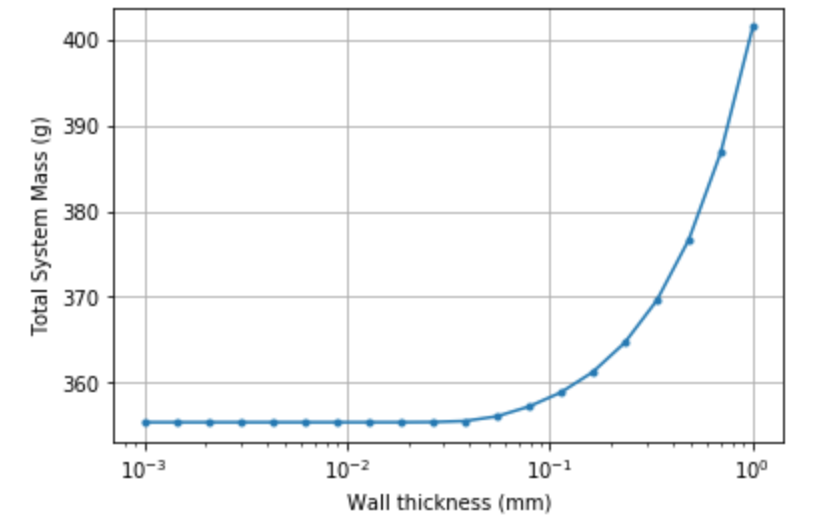
\includegraphics[width=0.5\linewidth]{sweep}
   \caption{Total system mass as we sweep over wall thicknesses}
   \label{fig:sweep}
\end{figure}
%FloatBarrier





\section{Conclusion}

Two systems were considered, one where Helium was stored at a high pressure, and fed through a regulator into a water tank with a diaphragm. The second system uses the self-pressurising combination of butane and propane, where the pressure can be controlled by tuning the temperature of the tank. This can be fine-tuned in the satellite using a feedback loop. 

The dry masses (excluding water, but including pressurants)  and internal tank volumes of the systems are summarised in Table~\ref{tbl:Summary}. We can see that the helium system uses less mass, however this figure neglects the mass of the regulator, pipes and extra structure. Helium has better flight heritage, but the self-pressurant system has fewer components, and is more compact.

\begin{table}[htbp]
   \centering
   \caption{Summary of various systems considered.}
   \begin{tabular}{@{} lcr @{}}
      \toprule
       Pressurant & Mass (g) & Tank Volume (cm$^3$)\\
      \midrule
Helium & 2.7 & 365.94 \\
Helium (constrained) & 11.3 & 373.33\\
\midrule
Butane and Propane & 5.4 & 355.84\\
Butane and Propane (constrained) & 13 & 355.84\\
      \bottomrule
   \end{tabular}
   \label{tbl:Summary}
\end{table}





\bibliographystyle{ieeetr}
\bibliography{biblio}


\end{document}























